\chapter{Implementation}
\label{chap:implementation}
\besk{Her presenterer jeg re-implementasjonen/etterlikningen/implementasjonsspesifikke-valg av K. Nymoens approach og teori i det nye systemet/simulatoren min i Unity — samt hvordan jeg har verifisert at mekanismene fungerer (e.g. fase-synkroniseringsplott)}

% Introducing the Chapter to what I've done/developed
This chapter gives an overview of the developed musical multi-robot system, methods implemented for it, as well as the performance measure used to evaluate these methods. The main goal of the implemented system is to allow for individual musical agents in a musical multi-agent collective to interact with each other, in order to achieve emergent and co-ordinating behaviour—in our case synchronization—with varying degrees of self-awareness, collective-sizes, and of difficulty and certainty in the environment and communication. More specifically, the goal with the design is to enable the robot collective to achieve so-called \textit{harmonic synchronization} within a relatively short time. Exactly what is meant by \textit{harmonic synchronization} will be expounded in Section \ref{sec:harmonic_synchrony}.

These goals firstly require of the agents the modelling of oscillators with their properties, like phase and frequency, as explained further in Subsection \ref{subsec:agent}. To allow for interaction and communication between the agents, mechanisms so that the agents can transmit "fire"-signals, as well as listen for other agents's "fire"-signals, is necessary as well, and is presented in Subsection \ref{subsec:fire_signal}.

First, the system and the system components will be presented and introduced. Then, methods implemented for achieving the system target goal of \textit{harmonic synchrony} in various synchronization objectives—firstly solely for oscillator-phases, then secondly for both oscillator-phases and oscillator-frequencies—will be described and presented. How the system target state of harmonic synchrony is detected will then be described in Section \ref{sec:performance_measure}.




% SEKSJON 1, Introducing my System and its System-components:
\section{Simulator setup: the musical multi-robot collective}
\label{sec:developed_system}
	\besk{Introduserer og presenterer det utviklede (simulator-)systemet du har utviklet i Unity selv, veldig gjerne med et fint Unity-/Simulator-system-skjema}

	Envision that we have a decentralized (i.e. no central control) multi-agent collective scenario consisting of musical robots modelled as oscillators. These are solely communicating through brief ``fire''-like audio-signals—greatly inspired by K. Nymoen et al.'s synchronizing ``fireflies'' \cite{nymoen_synch}. They are not initially synchronized in their firing of audio-signals; but as time goes, they are entraining to synchronize to each other by adjusting their phases and frequencies when/after hearing each other's audio-/fire-signals. If they then, after some time of listening to each other and adjusting themselves accordingly, succeed in becoming synchronized — we then will eventually see ``fire''-events/-signals line up at an even underlying pulse or rhythm. Examples and demonstrations of this process are depicted in Figure \ref{fig:first_idea:first_fig} and Figure \ref{fig:first_idea:second_fig}.

	% First Intro-illustration figure to easily get a quick idea of what the system/design does/consists of (to be exchanged with a describing system scheme/diagram):
	\begin{figure}[h]
	\centering
	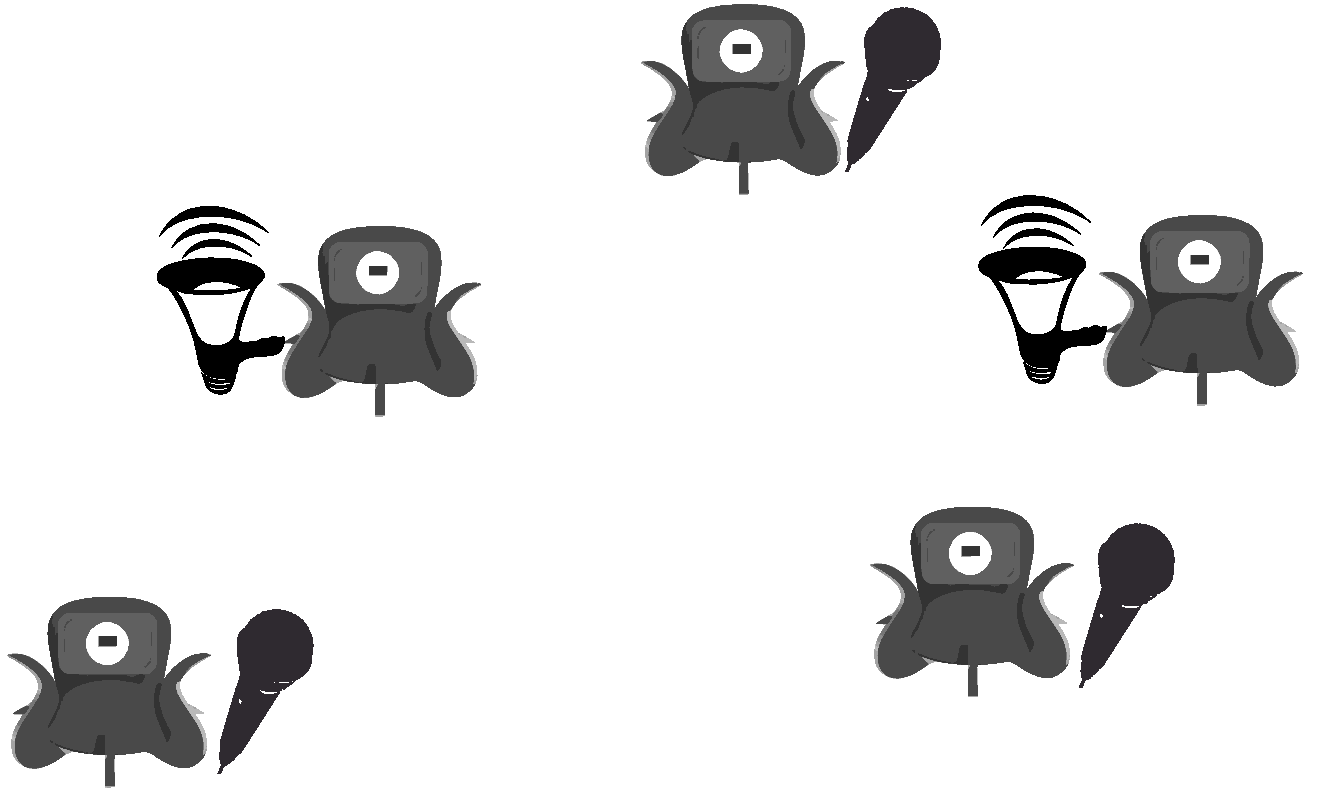
\includegraphics[width=0.9\linewidth]{Assets/Figures/schematic_initial_idea.pdf}
	\caption[Illustration/schematic of the developed multi musical robot collective/system]{Illustration/Schematic: The musical robot collective entraining to synchronize to each other, or more specifically to achieve harmonic synchronization, through performing phase- \& frequency-adjustments. Agents that are not firing at the moment will adjust themselves after hearing a transmitted ``fire''-/adjustment-signal from a neighbouring firing agent.}
	\label{fig:first_idea:first_fig}
	\end{figure}

	% Second Intro-illustration figure to easily get a quick idea of what the system/design does/consists of (to be exchanged with a describing system scheme/diagram):
	\begin{figure}[ht!]
		\centering
			\begin{subfigure}[t]{.5\textwidth}
				\centering\captionsetup{width=.9\linewidth}%
				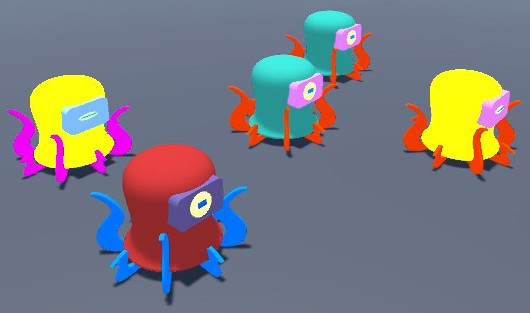
\includegraphics[width=0.9\linewidth]{Assets/Figures/Simulations/squiggles_unsynched_in_simulation.jpg}
				\caption{Screenshot from the very beginning of a Synchronization-simulation.}
				\label{fig:first_idea:second_fig:unsynched}
			\end{subfigure}%
			\begin{subfigure}[t]{.5\textwidth}
				\centering\captionsetup{width=.9\linewidth}%
				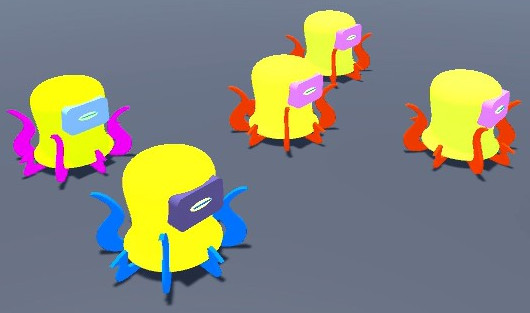
\includegraphics[width=0.9\linewidth]{Assets/Figures/Simulations/squiggles_synched_in_simulation.jpg}
				\caption{Screenshot from the same Synchronization-simulation as in \ref{fig:first_idea:second_fig:unsynched}, a few moments later.}
				\label{fig:first_idea:second_fig:synched}
			\end{subfigure}
		\caption[Synchronization-example/-screenshots from simulation in Unity]{From simulation: An example of the system target goal of harmonic synchrony being achieved in a musical robot collective, where oscillator-frequencies $\omega$ are constant and equal (1Hz), or in other words synchronized already, but oscillator-phases $\phi$ are unsynchronized and initially uniformly random numbers in the range of $[0,1]$. \nl
		At first in \ref{fig:first_idea:second_fig:unsynched}, we see the agents firing, i.e. blinking with their eyes and turning their body yellow, asynchronously at first. Only two robots, one with pink and one with red tentacles, fire synchronously so far. Seconds later in \ref{fig:first_idea:second_fig:synched}, after having listened to each others's adjustment-signals and adjusted themselves accordingly, all agents now fire simultaneously and synchronously.}
		\label{fig:first_idea:second_fig}
	\end{figure}

	% \inkl{Noe om hyperparameterne?}

	% INCLUDE PHASES UNSYNCHED VS. SYNCHED PLOT? See 'Relevant MSc-thesis Concerns'.
		% % Phase-/time-plot Figure with two Subplots. Subplot 1: phase-/time-plot when oscillators are unsynchronized. Subplot 2: phase-/time-plot when oscillators are synchronized
		% \begin{figure}[h]
			% \centering
				% \begin{subfigure}[t]{.5\textwidth}
					% \centering\captionsetup{width=.9\linewidth}%
					% 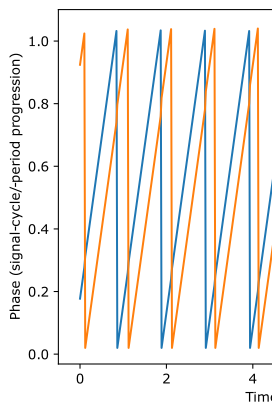
\includegraphics[width=0.9\linewidth]{Assets/Figures/phases_unsynched.png}
					% \caption{Oscillators are initially not (phase-) synchronized.}
					% \label{fig:phases_unsynched}
				% \end{subfigure}%
				% \begin{subfigure}[t]{.5\textwidth}
					% \centering\captionsetup{width=.9\linewidth}%
					% 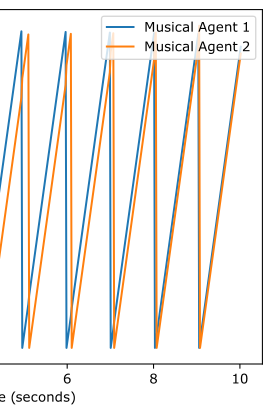
\includegraphics[width=0.9\linewidth]{Assets/Figures/phases_synched.png}
					% \caption{Oscillators are now, seconds later, (phase-) synchronized.}
					% \label{fig:phases_synched}
				% \end{subfigure}
			% \caption{Phase-plots for the agents}
			% \label{fig:initial}
		% \end{figure}



	% Introducing my own System Components:
	
	% Om den enkelte noden/agenten min med alle egenskaper den har osv.
	\subsection{The individual agent: a musical robot}
	\label{subsec:agent}
		As introduced and presented earlier, our musical robot collective will then consist of models of M. J. Krzyzaniak and RITMO's \textit{Dr. Squiggles}, 3D-models of which can be seen in Figure \ref{fig:first_idea:second_fig}.
	
		Every musical robot or node have certain components, attributes, and characteristics that make it what it is. Such include an oscillator-component, consisting of the agent's oscillator-phase $\phi$ and oscillator-frequency $\omega$. Notions like ``agent'', ``robot'', ``firefly'', and ``oscillator'' will be used interchangeably throughout the thesis. The agents have an input-mechanism for hearing/detecting transmitted ``fire''-event signals from other agents, as well as an output-mechanism for transmitting or playing such ``fire''-/adjust-signals or tones, as is illustrated with the microphone and megaphone respectively in Figure \ref{fig:first_idea:first_fig}.
		
		In order to be able to analyse the musical scenario within which they are situated (self-assessment), as well as for adapting their musical output accordingly (self-adaptation), the agents are to some extent endowed with artificial intelligence and self-awareness capabilities. The robots are self-aware of their own phase and frequency, but are unaware of other agents's true phases and frequencies. They also possess the self-assessment capability of evaluating how much in- or out-of-synch they are, as seen in the greater context of the entire robot collective. When the agents hear the transmitted ``fire''-/adjust-signals, the agents are intelligent enough to adjust themselves in the direction of the system goal/target state.


		
	% Om kommunikasjonen til agentene mine: audio-/``fire''-signalet
	\subsection{Robot communication: the ``fire''-signal}
	\label{subsec:fire_signal}
	
	These aforementioned audio-signals, also referred to as ``fire''-signals, ``flash''-signals, or adjust-signals, are transmitted whenever an agent's oscillator \textit{peaks} or \textit{climaxes} (i.e. after its cycle or period is finished, having phase $\phi(t)=1$) — or actually after every second \textit{peak}, as a way (discovered by K. Nymoen et al. \cite{nymoen_synch}) to attain the system target goal of \textit{harmonic synchrony}, to be elaborated upon in Section \ref{sec:harmonic_synchrony}.

	The ``fire''-signals are short and impulsive tones that the agents output through their loudspeakers. These short audio-signals/sounds ``wildly'' transmitted or played into the environment are then the only means of communication within the multi-agent collective, implying that are agents are pulse-coupled, not phase-coupled, oscillators. In other words, our agents will communicate and co-ordinate with each other through the very typical multi-agent system concept of \textit{stigmergy}.
	
	When an agent detects a ``fire''-/adjust-signal, the agent will adjust its own oscillator-properties (phase $\phi$ and frequency $\omega$), depending on which type of problem the agents are to solve. No individual agent is directly able to adjust or modify the state or properties of any other agent, only its own. Exactly the type of problems we attempt to solve in this thesis will be presented now in Section \ref{sec:phase_methods} and Section \ref{sec:frequency_methods}.
	
	\subsubsection{Under the hood in the simulator}
		\gjor{Fyll inn her med megafon-/mikrofon-pollingen hvis du implementerer det}
		Pretty basic and kinda like poking another robot immediately after a phase-climax.
	
	\subsubsection{Audible to human simulator-observer}
	
		\paragraph{Envelope-design}
		The fire-signal audible to the human observer watching and listening to the musical robots synchronizing to each other should be distinct and short enough so that one can clearly distinguish between which robots are firing and when. At the same time, the firing-sounds should to the human observer not be too sharp and loud to listen to so that it is uncomfortable observing the musical robot collective. Keeping these aspects in mind, some relatively soft and pleasant firing-sounds from an instrument usually associated with harmonious music—the harp—were produced and developed for the synchronization-simulator.
		
		Using the music-making system and digital synthesizer LMMS, some musical tones I thought sounded harmonious when played together (from the intro of Pogo's song ``Strangerous'') were digitally reproduced and recorded with a harp-instrument in LMMS, as can be seen in Figure \ref{fig:LMMS_harp}. 
		
		However, these harp-sounds sounds most like monotone and constant harp-pluckings, potentially making it hard to distinguish to the human ear when multiple robots are playing these frequently and simultaneously. The harp-sounds thus need to be slightly edited—which they in our implementation were in the audio-editing program Audacity—so that the long and constant harp-pluck became more of a ``quick'' and distinguishable ``sound-bullet'' — essentially what we want in a solid ``fire''-signal sound. The ``before'' (\textbf{(a)}) and ``after'' (\textbf{(b)}) of this audio-editing process is depicted in Figure \ref{fig:fire_signal_designing}. Edits performed on waveform \textbf{(a)} to obtain waveform \textbf{(b)} consists of effects like e.g. ``Fade Out'' (to dampen the sound in the tail of the waveform and get a shorter ``sustain''), ``Amplify'' (in order to get a as high ``attack''/max-amplitude as wanted to make the fire-sound audible enough) — and obviously cutting the waveform so that it is shorter (giving a ``quicker'' sound).
		
		\begin{figure}[!ht]
			\centering
			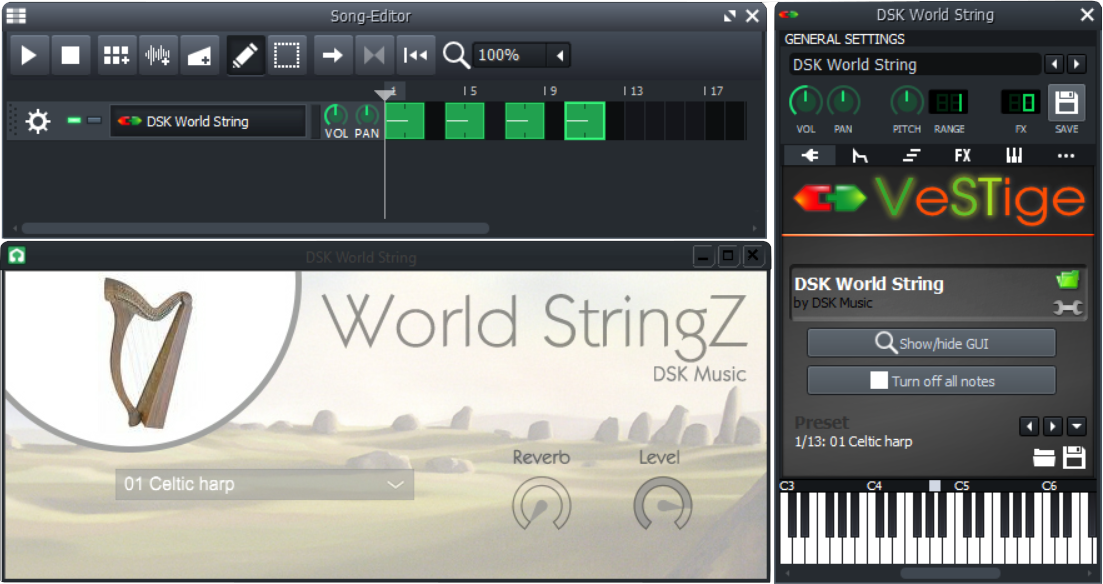
\includegraphics[width=\linewidth]{Assets/Figures/ToolOverview/LMMS_harp.png}
			\caption[Producing a digital harp-sound.]{Producing a digital harp-sound in the music-making and digital synthesizing program LMMS.}
			\label{fig:LMMS_harp}
		\end{figure}
		
		\begin{figure}[!ht]
			\centering
			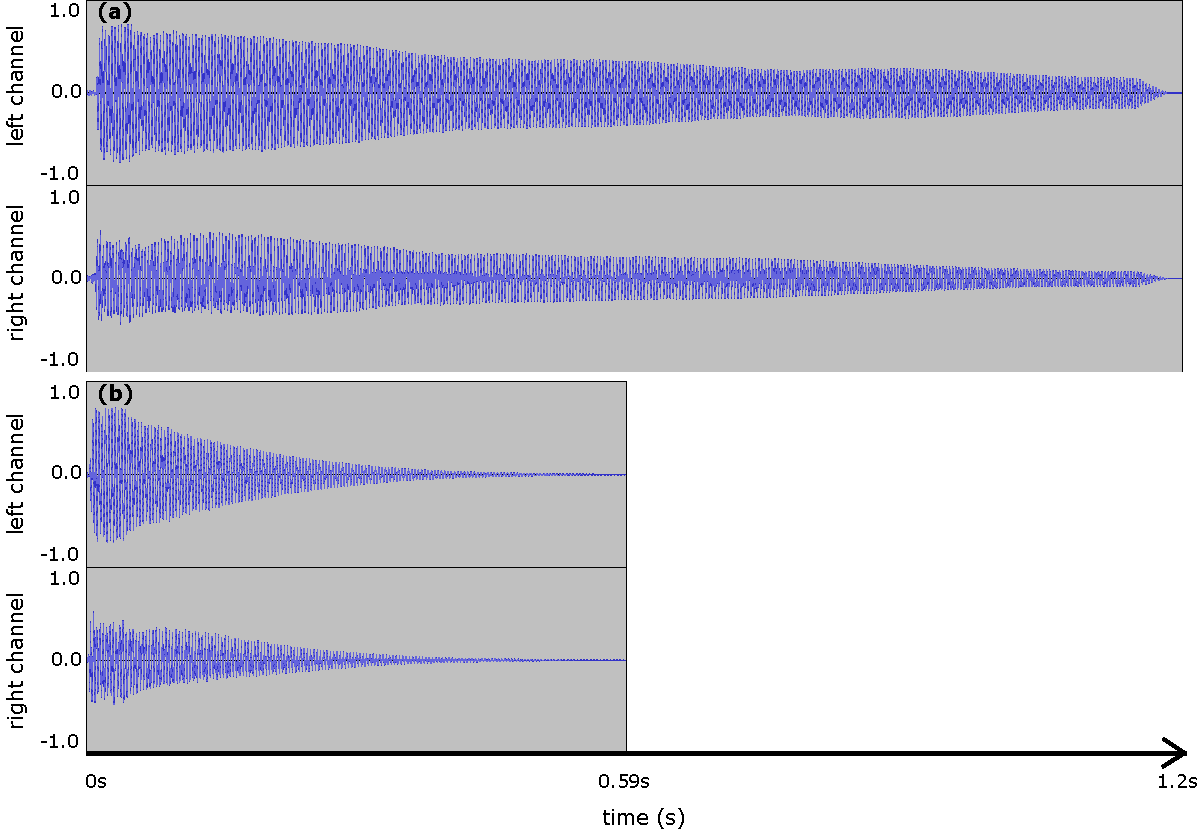
\includegraphics[width=\linewidth]{Assets/Figures/Illustrations/fire_signal_designing.pdf}
			\caption[Editing a pure harp-sound to become a fire-signal.]{Editing waveform \textbf{(a)}, being a ``raw'' harp plucking-sound, into waveform \textbf{(b)}, being a more distinguishable ``fire''-signal (although still sounding like a ``brief'' harp-sound).}
			\label{fig:fire_signal_designing}
		\end{figure}
	
	
		\paragraph{Frequency based fire-sound assignment}
		\besk{Presenting the assignment of firing-sounds, as developed in \textbf{Envelope-design}, (with varying fundamental frequencies) based on robot-frequencies}
		\inkl{Skisse som i Logs\&History-rM-notatet ditt kombinert med implementasjons-spesifikke detaljer som hvordan jeg fikk til å bytte}
	
	
	
	
% SEKSJON 2
% Presenting new Methods I implemented myself for Phase-Adjustment:
\section{Synchronizing oscillator-phases}
\label{sec:phase_methods}
	If we first assume constant and equal oscillator-frequencies in our agents, we can take a look at how the agents adjust their|initially random|phases in order to synchronize to each other. We will from here on and out refer to this first problem as \textbf{the $\phi$-problem}, given that the phases ($\phi_i$) for all agents $i$ are what we need to adjust and synchronize — and that frequencies ($\omega_i$) technically already are synchronized.
	
	The goal state of the agents is now for all agents to fire/flash simultaneously, after having started firing/flashing at random initially. Note that this is a special case of the final and ultimate goal of \textit{harmonic synchrony}. This is due to how all agents in the collective firing/flashing simultaneously, is considered having achieved harmonic synchrony since its phases would be synchronized if fire-events are lined up in even pulses, as well as all frequencies in the agent collective being within the set of ``legal'' frequencies, $\omega_{0} \cdot 2^{\mathbb{N}_0}$, where $\omega_0$ is the fundamental (smallest) frequency in the agent collective, and $0 \in \mathbb{N}_0$ — leading to $\omega_0 \cdot 2^0 = \omega_0$ to be a legal frequency, which is what all agents in our case here have as frequences.
	
	In order for the musical agents to synchronize to each other, they will have to—due to their heterogenous and randomly initialized phases—adjust or update their own phases according to some well-designed update-/adjustment-functions, as presented below.
	
	When it comes to the temporality and timing of when these updating functions are used and applied; Musical agents's phases get updated/adjusted immediately as ``fire''-/``flash''-events from neighbouring robots are perceived.
	
	
	
	% Mirollo-Strogatz's Phase-Adjustment
	\subsection{Verifying Mirollo-Strogatz's phase-adjustment} % used '-adjustment' before
	
	Mirollo-Strogatz's approach for synchronizing phases in oscillators, as introduced in \ref{mirollo_strogatz_phase_adjust}, is implemented in the Unity simulator, and each agent is endowed with \textbf{phase update function \eqref{strog_phase}} with which they adjust themselves according to when perceiving a ``fire''-signal as described above.
	
	The verification that this works in the newly built synchronization-simulator was performed by dumping all agents's phase-values $\phi(t)$ during simulation-runs. A plot of these $\phi(t)$-values, evolving through simulation-time in seconds, is shown in Figure \ref{fig:strog_phase}.
	
	\begin{figure}[h]
		\centering
		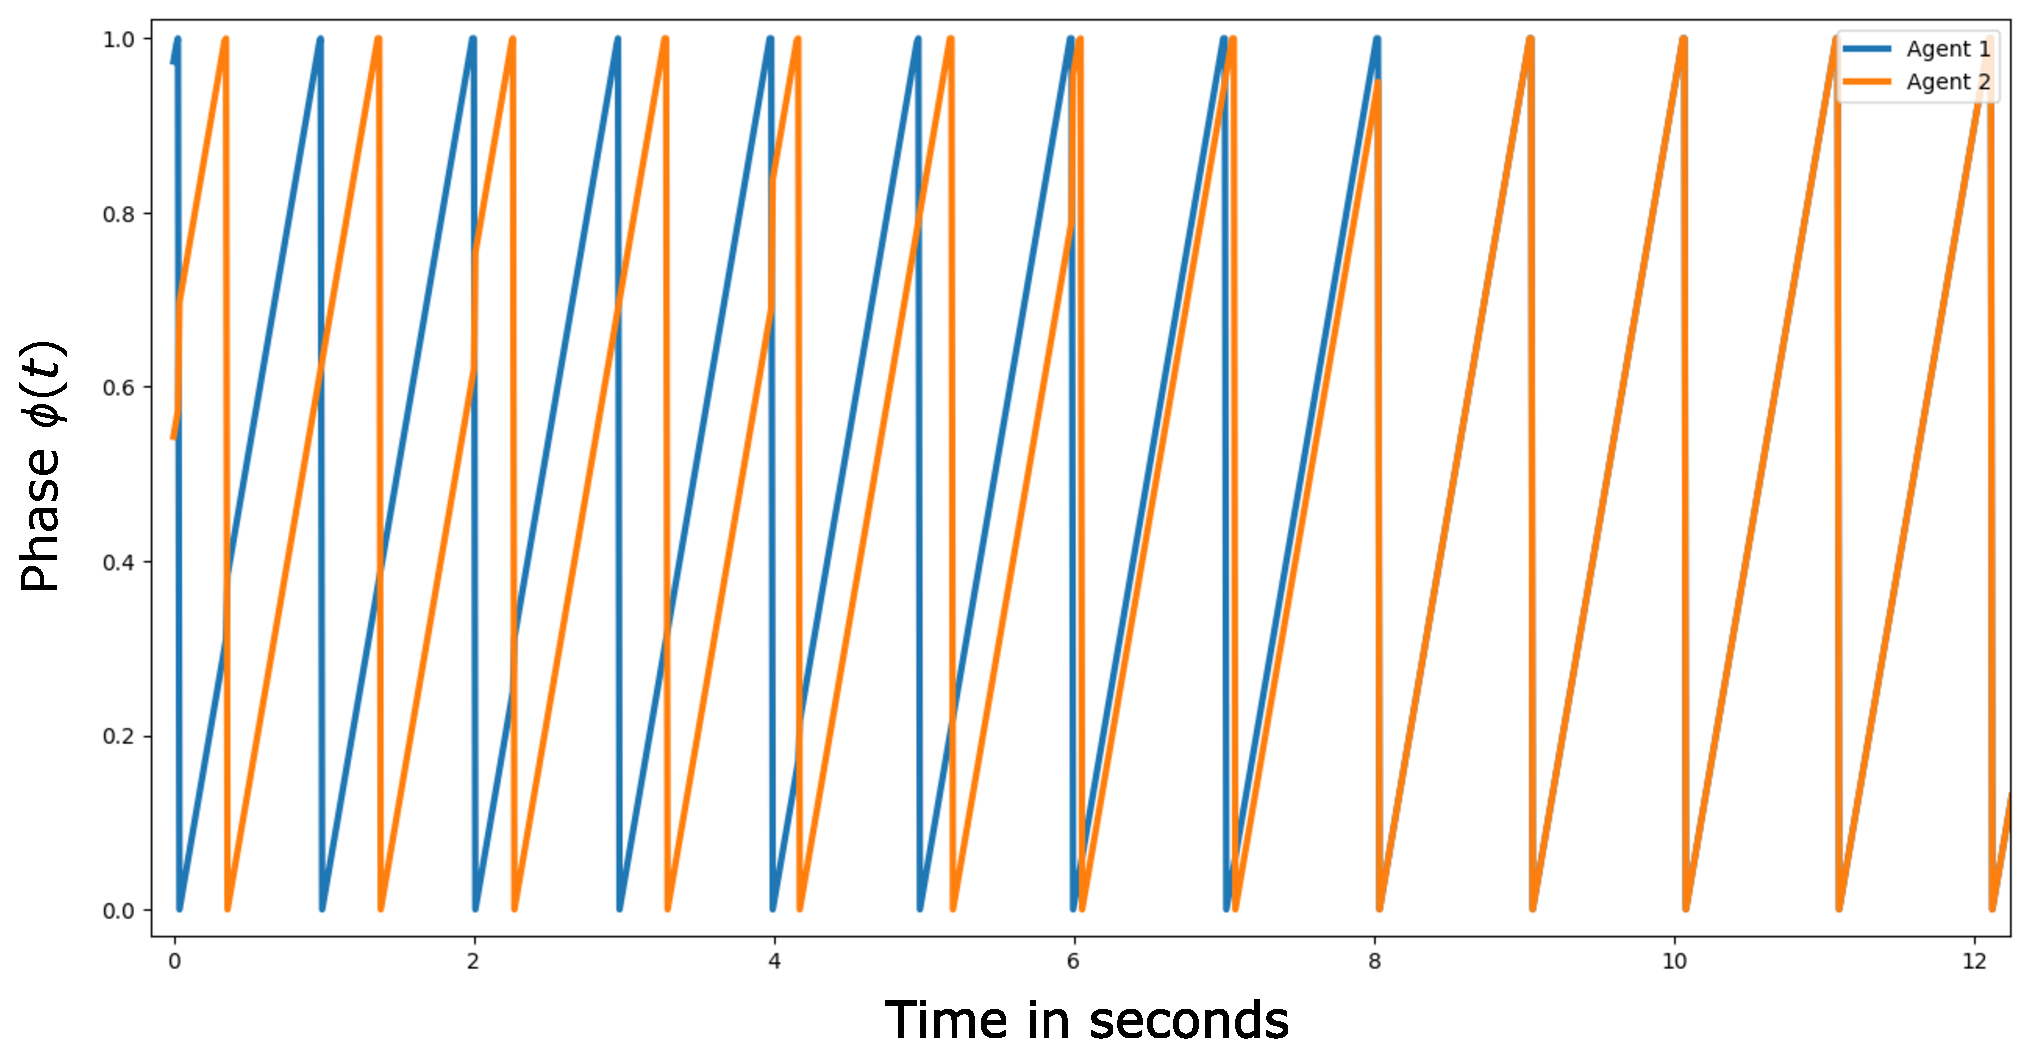
\includegraphics[width=0.9\linewidth]{Assets/Figures/MirolloStrogatzPhaseAdjustmentSecondTry.pdf}
		\caption[Illustration of Mirollo-Strogatz's ``standard'' phase-adjustment]{``Standard'' phase-adjustment with Mirollo-Strogatz's approach}
		\label{fig:strog_phase}
	\end{figure}
	
	
	
	% K. Nymoen's bi-directional phase-adjustment
	\subsection{Verifying K. Nymoen's bi-directional phase-adjustment} % used 'Shifts' before
	
	K. Nymoen et al.'s approach for synchronizing phases in oscillators, as introduced in Section \ref{nymoen_phase_adjust}, is implemented in Unity, and each agent is endowed with \textbf{phase update function \eqref{nymoen_phase}} with which they adjust themselves according to when perceiving a ``fire''-event as described above.
	
	The verification that this works in the newly set-up simulator-environment was performed by analysing carefully all the agents's phase-values $\phi(t)$ throughout a simulation-run. Such an analysis/plot can be seen in Figure \ref{fig:nymoen_phase}.
	
	\begin{figure}[h]
		\centering
		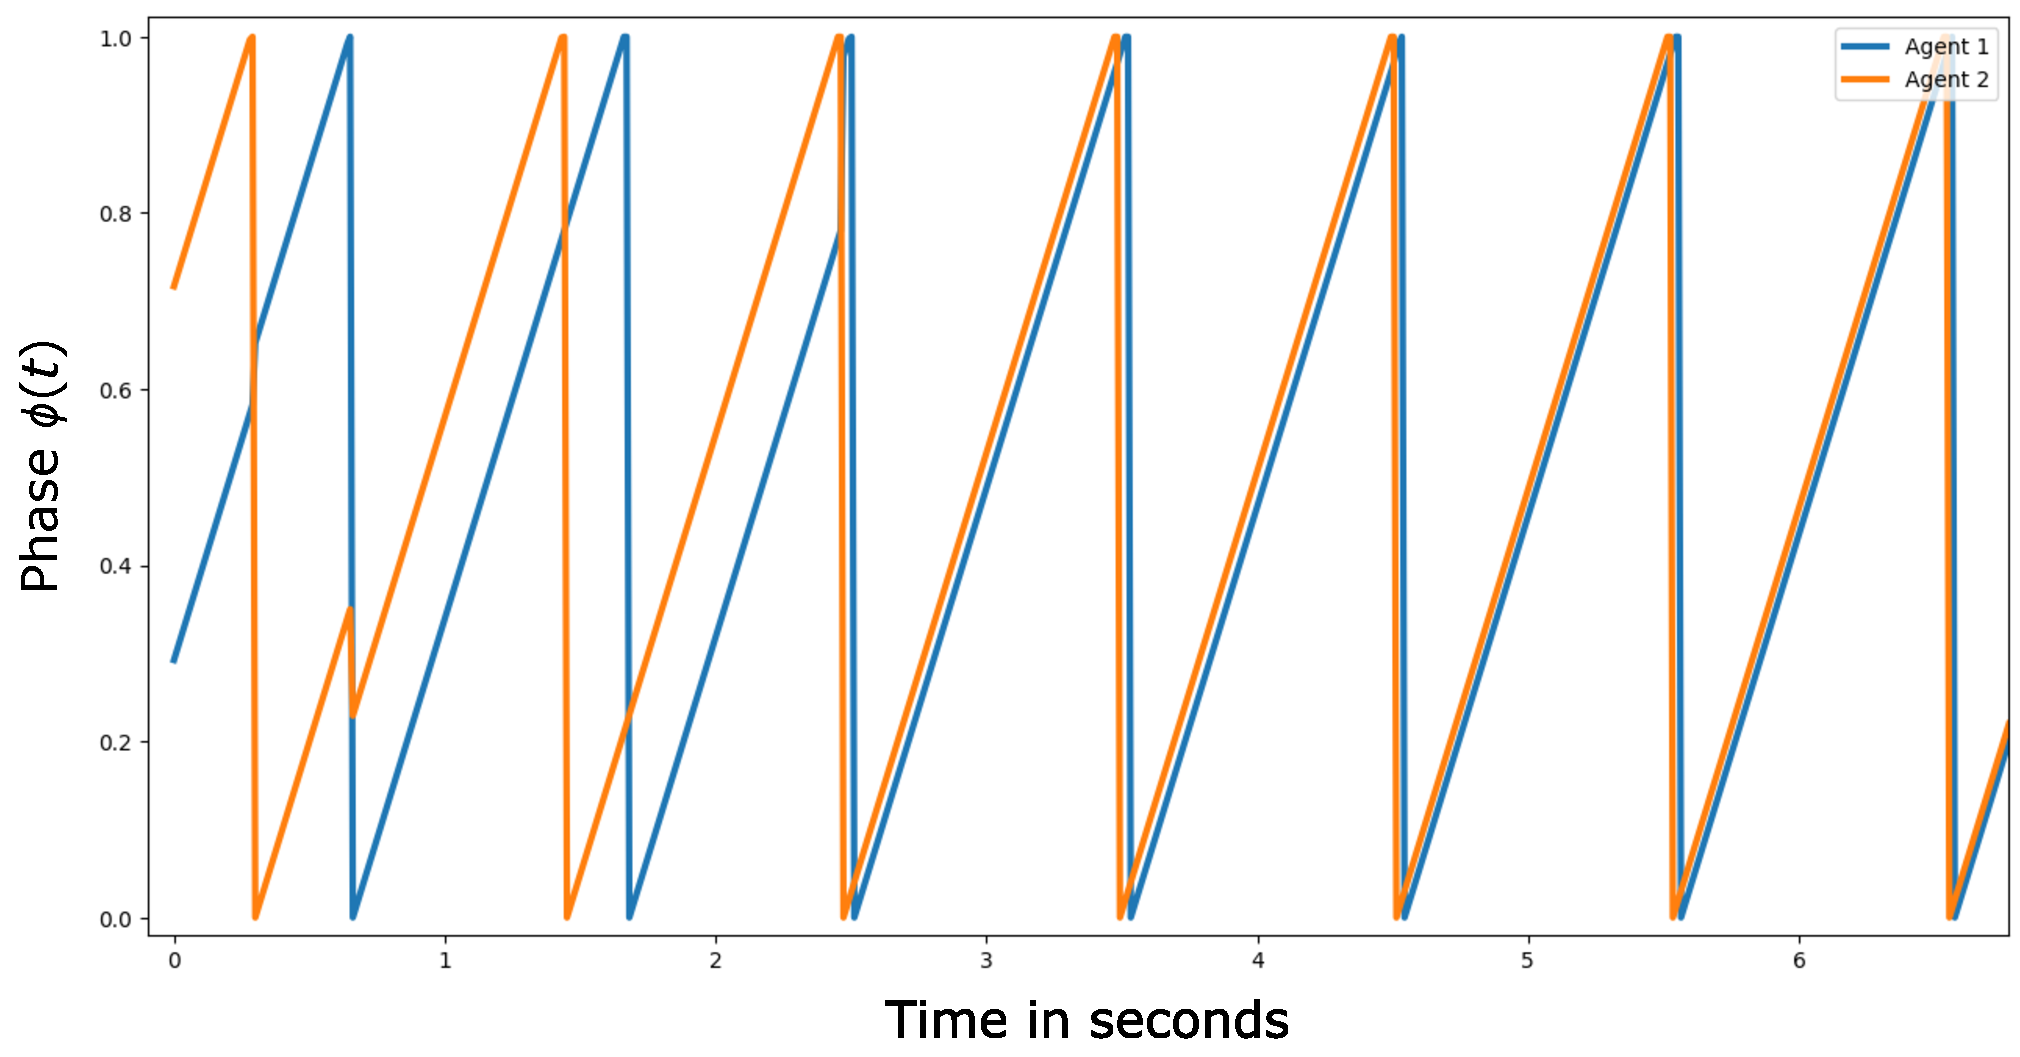
\includegraphics[width=0.9\linewidth]{Assets/Figures/KNymoenPhaseAdjustmentSecondTry.pdf}
		\caption[Illustration of K. Nymoen's bi-directional phase-adjustment]{Bi-directional phase-adjustment with K. Nymoen et al.'s approach}
		\label{fig:nymoen_phase}
	\end{figure}
	
	
	

	% PHASE.-ADJ APPROACH 3: HIGH LEVEL Self-Awareness
	% Hopefully an improved method with some additional Self-Awareness components
	\subsection{Thorvaldsen's self-aware phase-adjustment}
	
	\gjor{Beskriv min nye proposede algoritme (to-be-implemented) for å oppnå harmonisk synkronitet i $\phi$-problemet med phase-adjustment, som inneholder flere tilleggs- Self-Awareness-komponenter, sammenliknet med K. Nymoens bi-directional phase-adjustment metode. 
	
	Eksempler på slike tilleggs- Self-Awareness-komponenter er såkalt Belief-awareness (som fanger usikkerhet og tillits-nivåer) og/eller Expectation-awareness (som kombinerer Belief-awareness og Time-awareness) \cite{sacs17_ch3}. Andre forslag er å implementere Self-Awareness i forhold til:
	\begin{itemize}
		\item avstand: f.eks. $H^*(n)= H(n) \cdot \frac{1}{distance}$ for ``fire''-event $n$, så lenge ikke $distance = 0$.
		\item hvem som er hvem (i.e. agent\_id).
		% \item de andres frekvenser. Høre etter og registrere andre individers ``fire''-signaler kontinuerlig og estimere disse individenes frekvenser utifra det (f.eks. $\hat{\omega}_j = time_{j, fired\_now} - time_{j, fired\_last\_time}$, eller et gjennomsnitt av slike oppsamlede verdier).
	\end{itemize}
	}
	
	
	

% SEKSJON 3, Presenting new methods I implemented myself for frequency-synchronization:
\section{Synchronizing oscillator-frequencies}
\label{sec:frequency_methods}
	% Om Update-functions for frekvens-oppdateringene
	When we open up for the possibility for heterogenous frequencies in our musical agent collective, we open up to exciting musical aspects like the playing of diverse rhythmic patterns as e.g. mentioned in Section \ref{sec:harmonic_synchrony}, but we then also need to not only synchronize phases, but also frequencies, simultaneously. This second problem of adjusting synchronizing both all phases $\phi_i$ and frequencies $\omega_i$, the values of which can all be heterogenous and initially random, for all agents $i$ in the agent collective — we will from here on and out refer to as \textbf{the $\phi$-\&$\omega$-problem}. This slightly more complex problem calls for us to also find solutions on how to adjust and synchronize frequencies. We already have methods by which we can adjust and synchronize the agents's phases $\phi$ with, described in Section \ref{sec:phase_methods}, but we do so-far lack methods by which we can adjust and synchronize the agents's frequencies $\omega$ with.
	
	We hence now introduce randomly initialized, non-constant, and heterogenous oscillator-frequencies in our musical agents. The agents are now required to synchronize their initially different and random frequencies, so that frequencies are ``legal'' and \textit{harmonically synchronized}. Such ``legal'' frequencies are described clearly in detail in Section \ref{sec:harmonic_synchrony}.
	
	Some implemented approaches for achieving this are presented now. Notice the increasing degree of \textit{Computational Self-Awareness} endowed in the methods.
	
	
	% FREQ.-SYNCH APPROACH 2: MID LEVEL Self-Awareness
	% K. Nymoen's Frequency-Synchronization with some Self-Awareness
	\subsection{Verifying K. Nymoen's frequency-adjustment}
	
	In the newly proposed Unity simulator environment, the previously introduced self-assessed synch-score $s(n)$ (in \ref{s_n}) is implemented as a list containing \textit{m} error-scores $\epsilon$. Such a list is easily implemented in C\# by declaring a List$<$float$>$ called \textit{errorBuffer} e.g. (i.e. \textit{errorBuffer} is a list containing floating point values):
	
	\begin{equation}
	\label{error_buffer}
		errorBuffer = \{\epsilon(n), \epsilon(n-1), ... , \epsilon(n-m)\},
	\end{equation} \nl
	
	then leading to:
	
	\begin{equation}
	\label{self_assessed_synch}
		\begin{array}{rrclcl}
		s(n) & = & median(errorBuffer) \\ 
		& = & median(\{\epsilon(n), \epsilon(n-1), ... , \epsilon(n-m)\}) \in [0, 1],
		\end{array}
	\end{equation} \nl
	
	where $n$ is the latest observed ``fire-event'', and $m$ is the number of the last observed ``fire''-events we would like to take into account when calculating the self-assessed synch-score. \nl
	
	Regarding the ``frequency-update-contributions'' (the $H$-values described in \ref{H_n}) in my Unity-simulator, all the calculated H-values are accumulated and stored in an initially empty C\#-list (of floats), referred to as $H(n)$, at once they are calculated. The $H(n)$-list is then consecutively ``cleared out'' or ``flushed'' when its H-values have been used for the current cycle/period's frequency adjustment (i.e. at the phase climax, when $\phi(t)=1$), and is then ready to accumulate new H-values during the next cycle/period.
	
	
	% FREQ.-SYNCH APPROACH 3: HIGH LEVEL Self-Awareness
	% Hopefully an improved method with some additional Self-Awareness components
	\subsection{Thorvaldsen's high SA-leveled frequency-adjustment}
	
	\gjor{Beskriv min nye proposede algoritme (to-be-implemented) for å oppnå harmonisk synkronitet i $\phi$- \& $\omega$-problemet med frequency-adjustment, som inneholder flere tilleggs- Self-Awareness-komponenter, sammenliknet med K. Nymoens frequency-adjustment metode. Eksempler på slike tilleggs- Self-Awareness-komponenter er såkalt Belief-awareness (som fanger usikkerhet og tillits-nivåer) og/eller Expectation-awareness (som kombinerer Belief-awareness og Time-awareness) \cite{sacs17_ch3}. Andre forslag er å implementere Self-Awareness i forhold til, og vekte frekvensoppdaterings-bidragene H(n) i henhold til:
	\begin{itemize}
		\item avstand: f.eks. $H^*(n)= H(n) \cdot \frac{1}{distance}$ for ``fire''-event $n$, så lenge ikke $distance = 0$.
		\item hvem som er hvem (i.e. agent\_id).
		\item større median-liste ift. den self-assessed'e synch-score'n $s(n)$ og $errorBuffer$'et. Dette kan være nyttig ved større collective-sizes, da et lite/kort median-filter/-$errorBuffer$-liste vil kunne miste eller gå glipp av error-scores, $\epsilon(n)$, fra ``fire''-events fra langt tilbake (tidlig) i ``oppsamlings-perioden.''
		\item de andres frekvenser. Høre etter og registrere andre individers ``fire''-signaler kontinuerlig og estimere disse individenes frekvenser utifra det (f.eks. $\hat{\omega}_j = time_{j, fired\_now} - time_{j, fired\_last\_time}$, eller et gjennomsnitt av slike oppsamlede verdier).
	\end{itemize}
	}




% SEKSJON 4: Presenting the Performance-measure used to evaluate the implemented methods:
\section{Performance-/synchrony-measure: detecting harmonic synchrony}
\label{sec:performance_measure}

	The performance-measure will be used in our synchrony-simulator to evaluate and test the multi-robot collective's ability to harmonically synchronize to each other. As mentioned in Subsection \ref{subsec:harmonic_synchrony}, K. Nymoen et al.'s requirements and illustrations \cite{nymoen_synch} for achieving \textit{harmonic synchrony} serve as a blueprint or guide for how to similarly implement our synchrony-/performance-measure. This performance-measure should be able to, during synchronization-simulation, detect if harmonic synchronization has been achieved in our decentralized oscillator-network. The successful triggering of this detection will then in turn terminate the synchronization simulation-run and save to a dataset the time it took to synchronize (the performance-score), in the case of a `synchronization-success' — an example of which can be seen in Figure \ref{fig:perf_measure_plot}.

	\begin{figure}
		\centering
		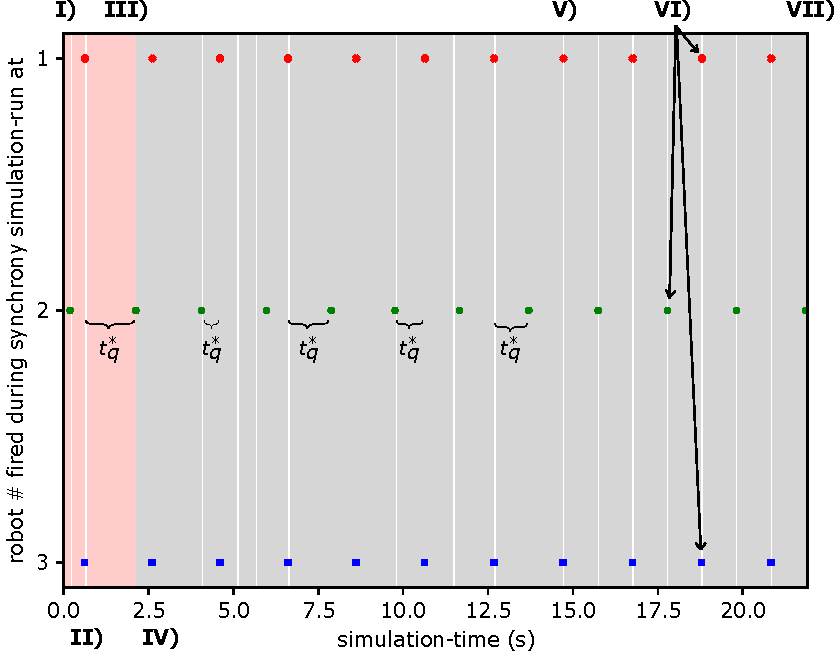
\includegraphics[width=\linewidth]{Assets/Figures/Illustrations/ExplanatoryIllustrativePerfMeasurePlot.pdf}
		\caption[A \textbf{performance-measure plot}.]{\textbf{Performance-/synchrony-measure plot}: recording a detection of harmonic synchrony. Initial red area represents the ``start-up''-period where no (gray) $t_q$-value is defined yet. \textbf{I)} First robot firing, initiating a process of defining such a ``silent'' time-window $t_q$ within which no nodes are allowed to fire, and a whole ``legal-firing'' $t_f$-window (here shaded in white and only 80ms long, as in \cite{nymoen_synch}) ensues. \textbf{II)} At least one robot firing, and with their firing-time(s) giving us the \textit{early $t_q$-defining} time-value (see schema below), as well as triggering second whole $t_f$-window to ensue. \textbf{III)} At least one robot firing after the \textit{early $t_q$-defining} time-value was found, hence (with their firing-time(s)) giving us the \textit{late $t_q$-defining} time-value right before using these when finishing the on-started process of defining the ``silent'' time-window $t_q$; triggering a half (due to stabilization purposes by future centering of fire-events) $t_f$-window to ensue. \textbf{IV)} A robot is caught firing illegally during a ``silent'' $t_q$-window and hence resets the \textit{towards\_k\_counter}-variable, as well as (re-) starts a process like in \textbf{I)} for (re-) defining a new $t_q$-value. \textbf{V)} Firing after this point only happens during short ``legal-firing'' $t_f$-windows, so \textbf{Condition 1} (cf. \ref{subsec:harmonic_synchrony}) is held. \textbf{VI)} All robots have fired at least once during the evaluation-period, so \textbf{Condition 2} is held. \textbf{VII)} The robot collective has fired legally and evenly, without resetting $t_q$, $k$ (equal to 8 in this case) times in a row, so \textbf{Condition 3} is fulfilled — and harmonic synchrony is thus achieved and detected after 21.9 seconds of synchronization.}
		\label{fig:perf_measure_plot}
	\end{figure}

	The resulting and corresponding performance-scores obtained using this perf-ormance-measure will then take values of the simulation-time (in seconds) it takes for the robot-collective, from the start of the synchronization-simulation, to achieve the system target state of \textit{harmonic synchrony}, as specified in Section \ref{sec:harmonic_synchrony}.

	Now if \textbf{Conditions 1-3} from Subsection \ref{subsec:harmonic_synchrony} are kept, we have harmonic synchrony.

	My specific implementation of the performance-/synchrony-measure essentially consists of enforcing all the requirements or rules listed in \ref{subsec:harmonic_synchrony}, given some constant $t_f$- and $k$-values (e.g. $80ms$ and $8$ respectively \cite{nymoen_synch}). And again—to recall from \ref{subsec:harmonic_synchrony}—$t_f$ is the short time-window within which nodes are allowed to fire at each beat, and $k$ represents how many times nodes have to fire at even underlying pulses/beats in a row without changing the $t_q$-period—before becoming harmonically synchronized.

	The requirement of firing evenly $k$ times in a row with identical $t_q$-periods can be—and in fact is in our implementation—enforced by incrementing an integer variable \textit{towards\_k\_counter} after a `legal' $t_f$-window has occured (i.e. one or more nodes fired inbetween the onset and ending of the $t_f$-window), and conversely by resetting \textit{towards\_k\_counter} to 0 when an illegally transmitted firing was heard during a `silent' (or so it was supposed to be at least) $t_q$-window, hence restarting the synchrony-detection process—as can be seen occuring several times in Figure \ref{fig:synch_evolution_perf_measure_ill}.

	\begin{figure}[h]
		\centering
		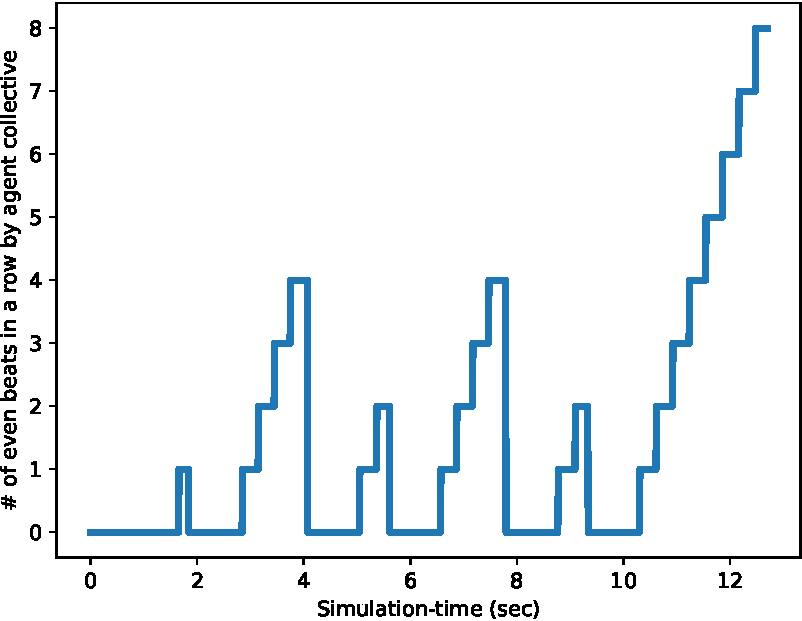
\includegraphics[width=0.85\linewidth]{Assets/Figures/Illustrations/SynchronyEvolutionPerfMeasureIllustration.pdf}
		\caption[A \textbf{synchrony-evolution plot}.]{A \textbf{synchrony-evolution plot}, displaying the temporal recording of the \textit{towards\_k\_counter}-variable throughout a synchrony simulation-run in Unity. The counter is incremented as the robot-collective fires evenly within `legal' $t_f$-windows, and is conversely reset to 0 if illegal firings during `silent' $t_q$-windows are heard. Note that in this specific simulation-run above, the agents were on their way to achieve harmonic synchrony five times before the 10th second of the synchronization-simulation already, but since one or more of them fired `illegally' (i.e. inside a $t_q$-window), they were consequently `punished'—or rather deemed `not synchronized enough yet'—by getting their counter reset to 0. Eventually however,  through further phase- \& frequency-synchronization, the multi-robot collective was in this case after 12.5 seconds able to achieve harmonic synchrony, when \textit{towards\_k\_counter} became equal to $k$, as well as all other requirements for achieving \textit{harmonic synchrony} was met.}
		\label{fig:synch_evolution_perf_measure_ill}
	\end{figure}

	Initially, the $t_q$-period/-window is not initialized, as it entirely depends on the frequencies to which the robot-collective converges to; however, when an illegal firing (i.e. a firing perceived during a $t_q$-window) occurs—$t_q$ is also then reset itself to a hopefully more correct value, given by the following formula, which is visually explained further in the schema in Figure \ref{fig:t_q_schema}:

	\begin{equation}
	\label{t_q_definition}
	\begin{array}{rrclcl}
	t_q^* & = & late\_t_q^*\_defining\_timevalue - early\_t_q^*\_defining\_timevalue - t_f \\
	& = & median(t_1^`, t_2^`, ..., t_m^`) - median(t_1, t_2, ..., t_n) - t_f , \\
	\end{array}
	\end{equation}

	where $n$ fire-events were recorded during the earlier $t_f$-window, and $m$ fire-events were recorded during the later $t_f$-window.


	\begin{figure}[ht!]
		\centering
		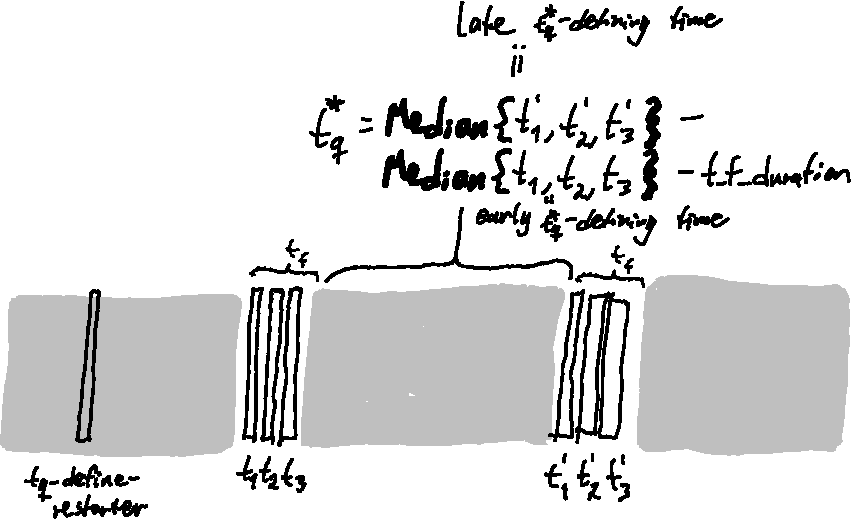
\includegraphics[width=0.85\linewidth]{Assets/Figures/Illustrations/t_q_schema.pdf}
		\caption{Schema: how ``silent'' $t_q$-windows are defined based on firing-times during $t_f$-windows. \tcol[red]{Til Kyrre: Dette var bare grovt, som jeg tenker jeg må lage mer profesjonelt i Inkscape ellernoe.}}
		\label{fig:t_q_schema}
	\end{figure}


	The specific steps and procedures needed to implement this performance-/synchrony-measure is expounded in detail in Algorithms \ref{perf_synch_measure_algo_A}, \ref{perf_synch_measure_algo_B}, and \ref{perf_synch_measure_algo_C}.

	\begin{algorithm}
	\caption{Performance-/synchrony-measure part A \tcol[red]{(må evt. fylles inn)}}\label{perf_synch_measure_algo_A}
	\end{algorithm}

	\begin{algorithm}
	\caption{Performance-/synchrony-measure part B \tcol[red]{(må evt. fylles inn)}}\label{perf_synch_measure_algo_B}
	\end{algorithm}

	\begin{algorithm}
	\caption{Performance-/synchrony-measure part C \tcol[red]{(må evt. fylles inn)}}\label{perf_synch_measure_algo_C}
	\end{algorithm}

	If a certain amount of time, e.g. 5 minutes \cite{nymoen_synch}, has gone without the detection of harmonic synchrony occuring, the simulation-run is terminated as a ``fail''.